\documentclass[tikz,border=10pt]{standalone}
\usepackage{tkz-euclide} % 增强几何绘图工具
\begin{document}
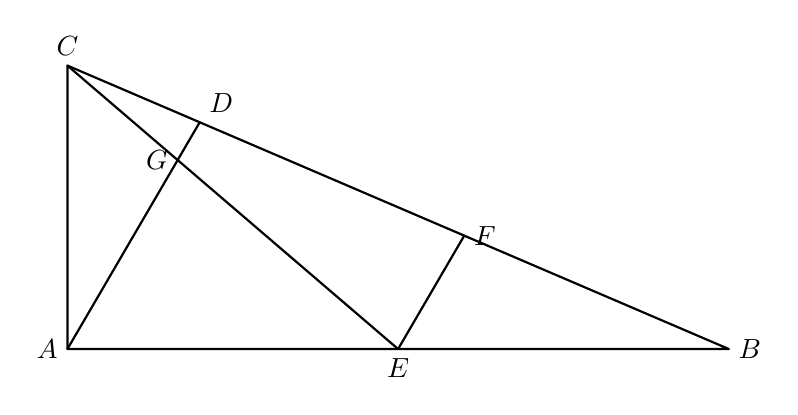
\begin{tikzpicture}[scale=1.2, line cap=round, line join=round]    
% 1. 定义核心顶点坐标 (基于图像比例估算)    
\coordinate (A) at (0, 0);    
\coordinate (B) at (7, 0);    
\coordinate (C) at (0, 3);        
% 2. 绘制主三角形 ABC    
\draw[thick] (A) -- (B) -- (C) -- cycle;        
% 3. 定义点 E (在 AB 上) 和 F (在 BC 上)    
\coordinate (E) at ($(A)!0.5!(B)$);    
\coordinate (F) at ($(C)!0.6!(B)$); % E, F 构成的线段与 BC 相关        
% 4. 计算并绘制线段 CE    
\draw[thick] (C) -- (E);        
% 5. 绘制线段 AD 并标出点 G, H    
% D 位于 BC 上    
\coordinate (D) at ($(C)!0.2!(B)$);    
\draw[thick] (A) -- (D);        
% G 是 AD 与 CE 的交点    
\coordinate (G) at (intersection of A--D and C--E);        
% 6. 绘制线段 EF    
\draw[thick] (E) -- (F);          
    % 8. 标注点名称    
% pos 控制标注位置，node 里的文字是 LaTeX 文本    
\node[left] at (A) {$A$};    
\node[right] at (B) {$B$};    
\node[above] at (C) {$C$};    
\node[above right] at (D) {$D$};    
\node[below] at (E) {$E$};    
\node[right] at (F) {$F$};    
\node[left] at (G) {$G$};
   
\end{tikzpicture}
\end{document}